% Part: history
% Chapter: set-theory
% Section: limits

\documentclass[../../../include/open-logic-section]{subfiles}

\begin{document}

\olfileid{his}{set}{limits}

\olsection{تعریف دقیق حد}

امروزه راه‌حل استاندارد مسئلهٔ پیش‌گفته کنارگذاشتن بی‌نهایت‌کوچک‌هاست.
روش کار چنین است.

دیدیم که هرچه $\beta$ کوچک‌تر شود، تقریب بهتری از شیب به دست می‌آید. در
واقع، هرچه $\beta$ به‌دلخواه به $0$ نزدیک شود، مقدار خارج‌قسمت تفاضلی
«بی‌حد نزدیک می‌شود» به شیبی که می‌خواهیم. بنابراین به‌جای بررسی آنچه
\emph{در} $\beta = 0$ رخ می‌دهد، کافی است \emph{روند} خارج‌قسمت تفاضلی را
هنگامی که $\beta$ به $0$ نزدیک می‌شود بررسی کنیم.

با این بیان، چالش کلی معنابخشیدن به گزاره‌هایی با صورت زیر است:
\begin{center}
وقتی $x$ به $c$ نزدیک می‌شود، $g(x)$ بی‌حد به $\ell$ میل می‌کند.
\end{center}
این گزاره را می‌توانیم به‌اختصار چنین بنویسیم:
\[
\lim_{x \rightarrow c}g(x) = \ell.
\]
در سدهٔ نوزدهم، وایرشتراس با تکیه بر کارهای پیشین کوشی تعریفی کاملاً دقیق
از این عبارت عرضه کرد. ایده این است که با نزدیک‌کردن مناسب $x$ به~$c$،
می‌توانیم $g(x)$ را هرقدر بخواهیم به~$\ell$ نزدیک کنیم. دقیق‌تر بگوییم،
مقرر می‌کنیم که $\lim_{x \rightarrow c} g(x) = \ell$ یعنی:
\[
(\forall\epsilon > 0)(\exists \delta > 0)\forall x
\left(0 < |x - c| < \delta \lif |g(x) - \ell| < \epsilon \right).
\]
خطوط عمودی در اینجا قدر مطلق را نشان می‌دهند. یعنی وقتی $x \geq 0$،
$|x| = x$، و وقتی $x < 0$، $|x| = -x$؛ نمودار \emph{این} تابع چنین
است:
\begin{center}
	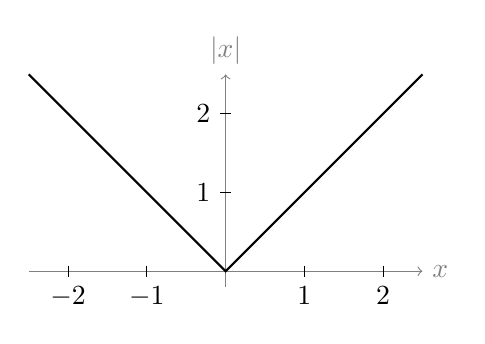
\begin{tikzpicture}[scale=1]
	\draw[->, gray] (-2.5,0) -- (2.5,0) node[right] {$x$};
	\draw[->, gray] (0,-.2) -- (0,2.5) node[above] {$|x|$};

	\foreach \x/\xtext in {-2/-2, -1/-1, 1/1, 2/2}
	\draw[shift={(\x,0)}] (0pt,2pt) -- (0pt,-2pt) node[below] {{$\xtext$}};

	\foreach \y/\ytext in {1/1, 2/2}
	\draw[shift={(0,\y)}] (2pt,0pt) -- (-2pt,0pt) node[left] {{$\ytext$}};

	\draw[thick] (-2.5, 2.5)--(0,0)--(2.5, 2.5);
	\end{tikzpicture}
\end{center}
پس تعریف، به‌تقریب، چنین می‌گوید: با انتخاب ورودی‌هایی که فاصله‌شان از
~$c$ کمتر از $\delta$ است (یعنی $|x-c|<\delta$)، می‌توانید «خطا» را کمتر
از $\epsilon$ کنید (یعنی $|g(x)-\ell|<\epsilon$).

پس از تعریف مفهوم حد، می‌توانیم بی‌نهایت‌کوچک‌ها را یکسره کنار بگذاریم و
مقرر کنیم که شیب $f$ در $c$ چنین به دست می‌آید:
\[
	{f}'(c) = \lim_{x \rightarrow 0}
\left(\frac{f(c +x) - f(c)}{x}\right)
\text{، اگر این حد وجود داشته باشد.}
\]
بااین‌حال، باید بدانیم چرا تعریف ما به قید «اگر این حد وجود داشته باشد»
نیاز دارد. برای مثالی ساده، $f(x)=|x|$ را در نظر بگیرید که نمودارش را
همین الآن دیدیم. آشکارا $f'(0)$ تعریف‌نشده است: اگر از «سمت راست» به $0$
نزدیک شویم، شیب همواره $1$ است؛ اگر از «سمت چپ» نزدیک شویم، شیب همواره
$-1$ است؛ پس حد تعریف‌نشده است. بنابراین می‌توان افزود که تابع~$f$ در
~$x$ \emph{مشتق‌پذیر} است اگر و تنها اگر چنین حدی وجود داشته باشد.

دیدیم چگونه با مفهوم \emph{حد} مشتق‌گیری را صورت‌بندی کنیم. با همین مفهوم
می‌توان ایدهٔ تابع \emph{پیوسته} را تعریف کرد. (بولتسانو عملاً تا سال
۱۸۱۷ به این نکته پی برده بود.) صورت‌بندی کوشی--وایرشتراس از پیوستگی چنین
است. به‌تقریب: تابع~$f$ در نقطه‌ای پیوسته است هرگاه اگر دقت معینی در خروجی
تابع بخواهید، بتوانید آن را با الزام دقتی معین در ورودی تضمین کنید.
دقیق‌تر: $f$ در $c$ پیوسته است هرگاه با میل‌کردن $x$ به صفر، تفاضل
$f(c+x)$ و $f(c)$ نیز به $0$ میل کند. به بیان دیگر، $f$ در $c$
\emph{پیوسته} است اگر و تنها اگر
$f(c) = \lim_{x \rightarrow c} f(x)$.

ادامه‌دادن بحث ما را به آنالیز حقیقی می‌کشاند، حال‌آنکه موضوع ما نظریهٔ
مجموعه‌هاست. پس باید درنگ کنیم و نتیجه را بگوییم. ریاضی‌دانان در سدهٔ
نوزدهم آموختند با توسل به مفهوم دقیقاً تعریف‌شدهٔ \emph{حد}، بدون
بی‌نهایت‌کوچک‌ها کار کنند.

\end{document}
